\author{Andrew Lim}
\title{Predicting film box office openings with Wikipedia}
\date{12 Jan 2013}

\documentclass[10pt]{article}

\usepackage{anysize}
\usepackage{graphicx}
\usepackage{multicol}
\usepackage{setspace}
\usepackage{url}

\marginsize{1in}{1in}{1in}{1.25in}
\onehalfspacing

\begin{document}

    \maketitle
    
    \section{Introduction: Wikipedia as a gauge of social interest}
    
    \begin{figure}[h]
        \centering
        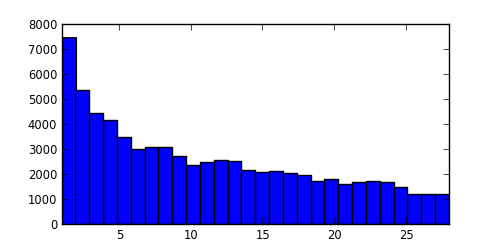
\includegraphics{wikipedia28.png}
        \caption{Count of Wikipedia article edits for the films used in this paper's training dataset over the 4 weeks prior each film's respective release date, bucketed by days before release date. This graph shows the uptick in editing activity that typically accompanies a film's release.}
    \end{figure}
    
    \paragraph{}
    According to its article on itself as of this writing, Wikipedia is ``a collaboratively edited, multilingual, free Internet encyclopedia'' launched in January 2011. Its articles can be edited by anyone, either anonymously (though the editor's IP address is logged) or with a registered user account. The edit history of each article is saved with a timestamp. Interested users can view any past version of an article, and an article's edit history exhibits an evolving record of Wikipedia's ``knowledge''\footnote{Of course, Wikipedia's highly open policy means both that it contains a stunning breadth of information from contributors with wide-ranging expertise and that said information is sometimes unreliable. For an example that was in the news not long before this paper was written, see \cite{bicholm}, or for Wikipedia's own list of Wikipedia hoaxes, see \cite{wikipedia-hoaxes}.} of its subject. 
    
    \paragraph{}
    As such, Wikipedia's edit history can be viewed as a barometer of social interest. For example, when a person is in the news, edit activity on his or her article often spikes. In fact, Wikipedia has template warnings indicating when an article is likely to be in flux due to a relevant current event. Edit activity on Wikipedia, in this sense, is akin to mentions on social networks like Facebook or Twitter, although perhaps with a smaller participating audience (although many people read Wikipedia, not nearly so many participate in its creation). 
    
    \paragraph{}
    One relatively standardized area where we can try to gauge the degree to which Wikipedia activity reflects social interest is in film box office performance. Films have relatively well-defined release dates prior to which we can measure activity on Wikipedia. They also have a well-defined, measurable outcome: revenues at the ticket booth. Theater owners obviously have a direct financial interest in knowing how well a film is going to perform. Advertisers and publicists, sellers of tie-in products, and film journalists have a slightly more indirect but still strong interest; they will want to know how they should spend their time and money. Can we use Wikipedia to usefully predict films' opening box office performances? 
    
    \section{Formulation of problem and data sources}
    
    \paragraph{}
    The specific question I set out to answer was: how accurately, using Wikipedia's help, can we predict the domestic per-theater box office gross of a film released widely in the US, over the first three days\footnote{Films traditionally open on Friday, and their ``opening'' often refers to their gross over the first Friday, Saturday, and Sunday that they are playing. However there are plenty of non-Friday openings as well. Consequently, I've stated the problem in terms of the first three days' worth of grosses.} of its release? 
    
    \paragraph{}
    The data sources I used to answer this question were: 
    
    \begin{itemize}
        \item Box Office Mojo (\url{http://www.boxofficemojo.com/}) - contains detailed box office data. I used it to select the universe of films that I would consider and as my source for theatrical release dates, number of opening theaters, and revenues. There is no API - the data was scraped with Beautiful Soup. 
        \item Rotten Tomatoes (\url{http://www.rottentomatoes.com/}) - a popular movie review aggregator. I used it to obtain descriptive information about films: genres, runtime, MPAA rating, cast and directors, and so on. It offers an API if you register for a key (which is free as of the present writing). 
        \item Wikipedia (English-language) (\url{http://en.wikipedia.org/}) - it also offers an API, no registration or key necessary. More accurately, the software package MediaWiki offers an API; Wikipedia is the best-known website running MediaWiki. 
    \end{itemize}
    
    \paragraph{}
    Much of the work involved in data retrieval and formatting was to ensure that data retrieved from these three sources corresponded to the same film; data from Rotten Tomatoes and Wikipedia was obtained by using their APIs' search functionalities, which can lead to incorrect hits if you are not careful. For example, we want to make sure that Rotten Tomatoes data for the 2012 film ``The Lucky One'' is not mapped to the 2008 film ``The Lucky Ones,'' or that for the 2010 film ``Salt'' we do not examine the Wikipedia article for salt, the mineral.\footnote{Box Office Mojo data had to be scraped from HTML, but the HTML was regular and consistent. Rotten Tomatoes has a nice JSON-based API for data retrieval, but its ranking of returns is quirky, sometimes retrieving obscure films or films with similar names (example: Oliver Stone's 2008 biopic ``W.'' was unfindable through search query, even through the website's front end; I had to go to Stone's Rotten Tomatoes page just to find the relevant web page). Wikipedia both has a nice API and solid/consistent lookup, which is all the more impressive given that it contains articles on anything, not just films.} 
    
    \paragraph{}
    The universe of films that I considered were those listed on Box Office Mojo as having opened in at least 1000 theaters. I manually excluded a handful of films that were re-releases or limited-engagement special features. I trained my algorithms on films released between 2007 and 2011, inclusive. In total, 689 films were in the training dataset. Data from films as far back as 2002 were used for some of the feature calculations; see the next section regarding similar-film performance. I tested my algorithm on films released in 2012, of which there were 124. 
    
    \section{Features}
    
    \subsection{Descriptive features}
    
    \paragraph{}
    Descriptive features considered were: year of release, runtime, MPAA rating, whether the film was released on a Friday or not, and membership in genres as defined by Rotten Tomatoes. Rotten Tomatoes has 18 genre labels, corresponding to typical film genres like ``drama,'' ``romance,'' and so on. A film can belong to any number of these genres. 
    
    \begin{figure}[h]
        \begin{multicols}{3}
            \begin{itemize}
                \footnotesize
                \item Action \& Adventure
                \item Animation
                \item Art House \& International
                \item Classics
                \item Comedy
                \item Cult Movies
                \item Documentary
                \item Drama
                \item Horror
                \item Kids \& Family
                \item Musical \& Performing Arts
                \item Mystery \& Suspense
                \item Romance
                \item Science Fiction \& Fantasy
                \item Special Interest
                \item Sports \& Fitness
                \item Television
                \item Western
                \normalsize
            \end{itemize}
        \end{multicols}
        \caption{Rotten Tomatoes genres.}
    \end{figure}
    
    \subsection{Wikipedia-based features}
    
    \paragraph{}
    For each Wikipedia article, I measured the number of ``edit runs'' that had occurred 0 to 7 days prior to midnight on the day of the film's release and also 7 to 28 days prior. I defined an edit run as a sequence of consecutive edits from the same author (identified by IP address if anonymous). Sometimes on Wikipedia the same author commits several edits in a row, presumably as part of a single effort to edit the page, which I wanted to correspondingly treat as a single edit. (This did in fact improve the results slightly compared to using the raw number of edits.)
    
    \paragraph{}
    I also checked the 28-day history of article revisions for certain expressions that might indicate something about a film's box office's performance. One feature used was the average number of instances of the word ``IMAX'' (case-insensitively searched). Another was the number of instances of JPEG image tags. Another was the number of headings and subheadings present in the article. 
    
    \subsection{Revenues of similar films}
    
    \paragraph{}
    I also included the opening revenue per theater of any ``similar'' films that had been released within the five years preceding a film's release. This was an attempt to capture the fact that a very reasonable approach toward predicting the revenue of a film is to take a look at comparable films; in particular, the natural benchmark for a sequel is its predecessor(s). The five-year bound was an arbitrary but reasonable window of data to consider; ``sequels'' that are separated by a large amount of time may not be particularly useful in any case. This is why I ended up using some data points as far back as 2002, even though the training set only extended back to 2007. 
    
    \paragraph{}
    I defined a film as ``subsequent'' to an older film (released in the five years previous) if they shared at least three common names amongst the cast members and the director, with collaborating directors treated as a single person (so the Coen brothers, for example, are treated as a single unit). Note that subsequence is directional, only using older films as input to newer films; it doesn't make sense to try to predict ``Spider-Man 2'' based on ``Spider-Man 3'' data. The feature that I used in the algorithms was average revenue of any subsequent films. (try different types of subsequence scoring...)
    
    \paragraph{}
    (illustration of some similarity scores, genre similarity)
    
    \subsection{Cross terms}
    
    \paragraph{}
    The best way to represent the impact of a boolean such as genre membership or MPAA rating may not be to consider it as a constant term but to consider the multiplying impact it has on other variables. Therefore, I also considered cross-terms between the boolean and the non-boolean features. 
    
    \section{Analysis and prediction on 2012 films}
    
    \paragraph{}
    A few different prediction algorithms produced similar results; the one that proved the most effective on the test set, as measured by $R^2$, was gradient boosting trees, although random forests and ordinary linear regression were not too far behind. (discussion on gradient boosting trees) Gradient boosting trees also have the nice feature of being relatively resistant to over-fitting, useful here because we can conceivably create a large number of features on this dataset without strong foreknowledge or expectation about their predictive power. 
    
    \paragraph{}
    Replicate train and test error graphs and significance
    
    \paragraph{}
    (alternative approaches, such as GLM)
    
    \section{Comparison to other predictions}
    
    \section{Conclusion}
    
    \section{References and resources}
    
    \subsection{Data sources}
    
    \subsection{Software packages}
    
    \subsection{Bibliography}
    
    \begingroup
    \renewcommand{\section}[2]{}  % removes the header - thanks to http://tex.stackexchange.com/questions/22645/hiding-the-title-of-the-bibliography
    \begin{thebibliography}{1}
        
        \bibitem{bicholm} Pfeiffer, Eric (4 Jan 2013). ``War is over: Imaginary `Bicholm' conflict removed from Wikipedia after five years.'' Retrieved 10 Jan 2012. \url{http://news.yahoo.com/blogs/sideshow/war-over-imaginary-bicholim-conflict-page-removed-wikipedia-234717353.html}
        
        \bibitem{wikipedia-hoaxes} ``List of hoaxes on Wikipedia.'' Retrieved 10 Jan 2012. \url{http://en.wikipedia.org/wiki/Wikipedia:List_of_hoaxes_on_Wikipedia}
        
    \end{thebibliography}
    \endgroup
    
\end{document}